\documentclass[output=paper]{langsci/langscibook} 
\ChapterDOI{10.5281/zenodo.1493293}
\author{Bianca Prandi\affiliation{University of Mainz}}
\title{An exploratory study on CAI tools in simultaneous interpreting: Theoretical framework and stimulus validation}
% \chapterDOI{} %will be filled in at production

\shorttitlerunninghead{An exploratory study on \textsc{cai} tools in simultaneous interpreting}

%\epigram{Change epigram in chapters/01.tex or remove it there }
\abstract{The acquisition of terminology and specialized knowledge prior to a technical conference represents a fundamental phase in the interpreter’s workflow, but quick and easy access to terminological information during the interpreting task is\linebreak equally important to support the interpreter in the rendition of terminology and to ensure a high-quality interpreting performance. 

Over the past few years, terminology management tools have been developed\linebreak specifically for interpreters, but the impact of such tools on the cognitive processes involved in simultaneous interpreting is still unclear. To this end, an exploratory study was conducted to evaluaonference interpreters were covered.te the appropriateness of the stimuli adopted for data collection and to verify whether the use of computer-assisted interpreting tools causes saturation or, on the contrary, helps prevent it by reducing the local cognitive load during terminology search and delivery of the target text.}
\maketitle

\begin{document}


\section{Introduction}\label{sec:prandi:1}
Computer-Assisted Interpreting (\textsc{cai}) emerged around 10 years ago to provide interpreters with tools to prepare for specialized events and to support them along the individual phases of their workflow, from preparation, to interpretation proper, to follow-up work after the assignment. \textsc{cai} tools thus rationalize the interpret\-er’s terminology work by making preparation more efficient and ultimately aim at improving the quality of the interpreter’s output, at least in terms of terminological precision and adequacy. \citet{Rütten2007} and \citet{Will2009} developed a theoretical model of the interpreter’s preparation work and laid the foundations for how a \textsc{cai} tool should be structured in order to address the specific needs of conference interpreters, which are mainly linked to the online nature of interpreting and the time constraints it entails.

To date, the number of \textsc{cai} tools available to interpreters is limited and their functionalities do not always cover all the phases of the interpreting process. \citet{Fantinuoli2018} distinguishes between first-generation and second-generation \textsc{cai} tools. The first (e.g. Interplex\footnote{\url{http://www.fourwillows.com/interplex.html}} and Terminus\footnote{\url{http://www.wintringham.ch/cgi/ayawp.pl?T=terminus}}) are ``designed to manage multilingual glossaries in an interpreter-friendly manner'' \citep[164]{Fantinuoli2018}, but do not offer an advanced search algorithm. The latter ``offer advanced functionalities that go beyond basic terminology management, such as features to organize textual material, retrieve information from corpora or other resources, learn conceptualized domains, and advanced search functions'' \citep[164]{Fantinuoli2018} and include Intragloss\footnote{\url{http://intragloss.com}} and InterpretBank\footnote{\url{http://www.interpretbank.com}}. Interpreter’s Help\footnote{\url{https://interpretershelp.com}} can also be considered a second-generation \textsc{cai} tool, as it implements an advanced search function through its companion tool Boothmate\footnote{\url{https://interpretershelp.com/boothmate}}. 

Following the recent introduction of these tools on the market, first attempts at an evaluation have been made. Two main trends can be identified in this respect. The most recent one focuses on developing a set of criteria against which the tools can be evaluated \citep{Costa2016, Will2015}. This approach is certainly ambitious, but it remains somewhat arbitrary. The evaluation criteria mainly reflect the features offered by the tools, but do not consider how they influence the product of the interpreting process in terms of terminological quality and whether they optimize the interpreters’ preparation and facilitate their work in the booth, by making the online retrieval of terminological units easier and improving the terminological quality. While the number and type of features of \textsc{cai} tools certainly is of interest for practitioners, the main reason for choosing to use \textsc{cai} tools, and to prefer one tool to the other ones available, should be the ability of such tools to positively influence the interpreter’s work in terms of cognitive capacity and, ultimately, quality. 

This is where the second trend in the evaluation of \textsc{cai} tools comes into play. Soon after the development of the first \textsc{cai} tools, the first studies on the topic appeared. Apart from a few Master’s theses, which are limited in scope and often take a descriptive approach rather than an investigative one (see for example \citealt{DeMerulis2013}), a rather small number of publications can be found which mostly deal with the application of \textsc{cai} tools to the preparation phase \citep{Xu2015, Fantinuoli2017a}. When it comes to the use of \textsc{cai} tools in the booth, the number of studies is very limited, as is their scope. First attempts at an empirical analysis of the use of \textsc{cai} tools during simultaneous interpreting (\textsc{si}) can be identified in \citet{Prandi2015a, Prandi2015b} and  \citet{Biagini2015}. These initial investigations of the issue speak in favor of the usability of \textsc{cai} tools and seem to suggest that they do improve the terminological quality of \textsc{si}. Both experiments were based on a product-oriented analysis of the test subjects’ deliveries. Biagini also included a statistical analysis of transcription data. Apart from these initial analyses, no empirical methodology has been tested in a wide-ranging experiment which implements psycho-physiological, process-oriented methods in addition to product-based analysis. Moreover, \citet{Fantinuoli2017b} recently addressed the topic of the integration of automatic speech recognition (\textsc{asr}) in \textsc{cai} tools for use in the booth.

A PhD research project underway at the Johannes Gutenberg University of Mainz\slash Germersheim \citep{Prandi2016, Prandi2017a, Prandi2017b} aims at bridging this research gap. By triangulating eye-tracking data and the analysis of the test subjects’ transcriptions, the project aims at providing a picture not only of the usability of \textsc{cai} tools during simultaneous interpreting, but also of the local variations in Cognitive Load (\textsc{cl}) and of the terminological quality of simultaneous interpretation performed with the support of a \textsc{cai} tool when compared to more traditional terminology management solutions. Through the study, I hope to develop a research methodology that can be used to evaluate \textsc{cai} tools and provide the much-needed empirical data that will be helpful not only to practitioners in choosing the best tool, but also to software developers, by highlighting potential shortcomings.

After discussing the theoretical framework of my analysis (\sectref{sec:prandi:2}), I present the research desiderata and the structure of an exploratory study conducted to test my research methodology (\sectref{sec:prandi:3}). \sectref{sec:prandi:4} describes the rationale behind the stimuli used in the experiment and the features of the speeches used. I then present the results of the analysis of the transcriptions (\sectref{sec:prandi:5}), which I use to evaluate the appropriateness of the stimuli. In the conclusions, I address future work and provide suggestions for further research.

\section{Theoretical framework}\label{sec:prandi:2}
In the investigation of simultaneous interpreting performed with the support of \textsc{cai} tools, my aim is not only to look at the product of such activity, but also at the process that lies behind it. For this reason, in establishing a theoretical framework for my analysis, I took into consideration the two theoretical models that set out to describe interpreting from a procedural point of view and that address the allocation of cognitive resources during this very complex mental activity: Gile’s Effort Model (\textsc{em}) and Seeber’s Cognitive Load Model (\textsc{clm}) of simultaneous interpreting. In this section, I discuss why Seeber’s approach is more suited to the operationalization of my hypotheses.

\subsection{Gile’s Effort Model and Seeber’s Cognitive Load Model of simultaneous interpreting}\label{sec:prandi:2.1}
The main point of divergence between Gile’s Effort Model \citep{Gile1988, Gile1997, Gile1999} and Seeber’s Cognitive Load Model lies in the theoretical assumptions they stem from. Gile draws from Kahneman’s single resource theory \citep{Kahneman1973}\linebreak which does not find much validation in scientific literature. If there is one single pool of resources interpreters can adopt, how can some interpreters perform a terminological search on the Internet, while at the same time delivering a perfectly acceptable rendition of the original speech? This kind of multi-tasking might seem impossible to a first-year interpreter trainee, but is commonly observed among experienced professional interpreters. The second controversial assumption is that interpreters work close to saturation level most of the time (\citeauthor{Gile1999}’s ``tightrope hypothesis'', \citeyear{Gile1999}). While this might be true in some cases, for instance when the source speech is particularly dense, fast, or pronounced with a non-native accent, there might very well be cases in which the interpreter has enough spare cognitive resources to do something else while interpreting. 

In his Cognitive Load Model of simultaneous interpreting, Seeber takes an opposite approach to Gile’s, basing his model on Wickens’s multiple resource theory and on his Cognitive Load Model (\citeyear{Wickens1984, Wickens2002}). Wickens developed his model to account for the fact that qualitative differences in tasks being performed at the same time lead to ``differences in time-sharing efficiency'' \citep[162]{Wickens2002}, as shown by \citeauthor{Kantowitz1976} (\citeyear{Kantowitz1976}) and Wickens (\citeyear{Wickens1976}) himself. According to Wickens, different kinds of tasks require resources that are managed by discrete structures. When two or more tasks are performed simultaneously and ``all other things [are] equal (i.e. equal resource demand or single task difficulty), two tasks that both demand one level of a given dimension (e.g. two tasks demanding visual perception) will interfere with each other more than two tasks that demand separate levels of the dimension (e.g. one visual, one auditory task)'' \citep{Wickens2002}. In other words, performing a visual and an auditory task simultaneously will be ``easier'' (i.e. more efficient), because the underlying structures are not shared, than performing two visual tasks, as they share the same structures. In his model, Wickens identifies four dimensions, each made up of two ``levels'':
\begin{itemize}
\item processing stages (perception \& cognition\footnote{Perception and cognition are considered as one dimension, as one cannot take place without the other.}\slash responding)
\item processing codes (spatial\slash verbal)
\item processing modalities (visual\slash auditory)
\item visual processing (ambient\slash focal)
\end{itemize}

Not shown in the graphic representation of the model (\figref{fig:prandi:1}), but postulated by Wickens, is an additional pool of general capacity, which is always available to all tasks. In his adaptation of Wickens’s model to simultaneous interpreting, Seeber takes a step further, simplifying the graphical representation of Wickens’s model by turning it into a \textsc{2d} model (see \figref{fig:prandi:2}). This has two main advantages. First, it allows seeing all ``sides'' of the cube (i.e. all dimensions) at once. Second, it graphically introduces the general capacity left out in Wickens’s ``cube''. 

\begin{figure}
	%%please move the includegraphics inside the {figure} environment
	%%\includegraphics[width=\textwidth]{Ch2-img9.png}
	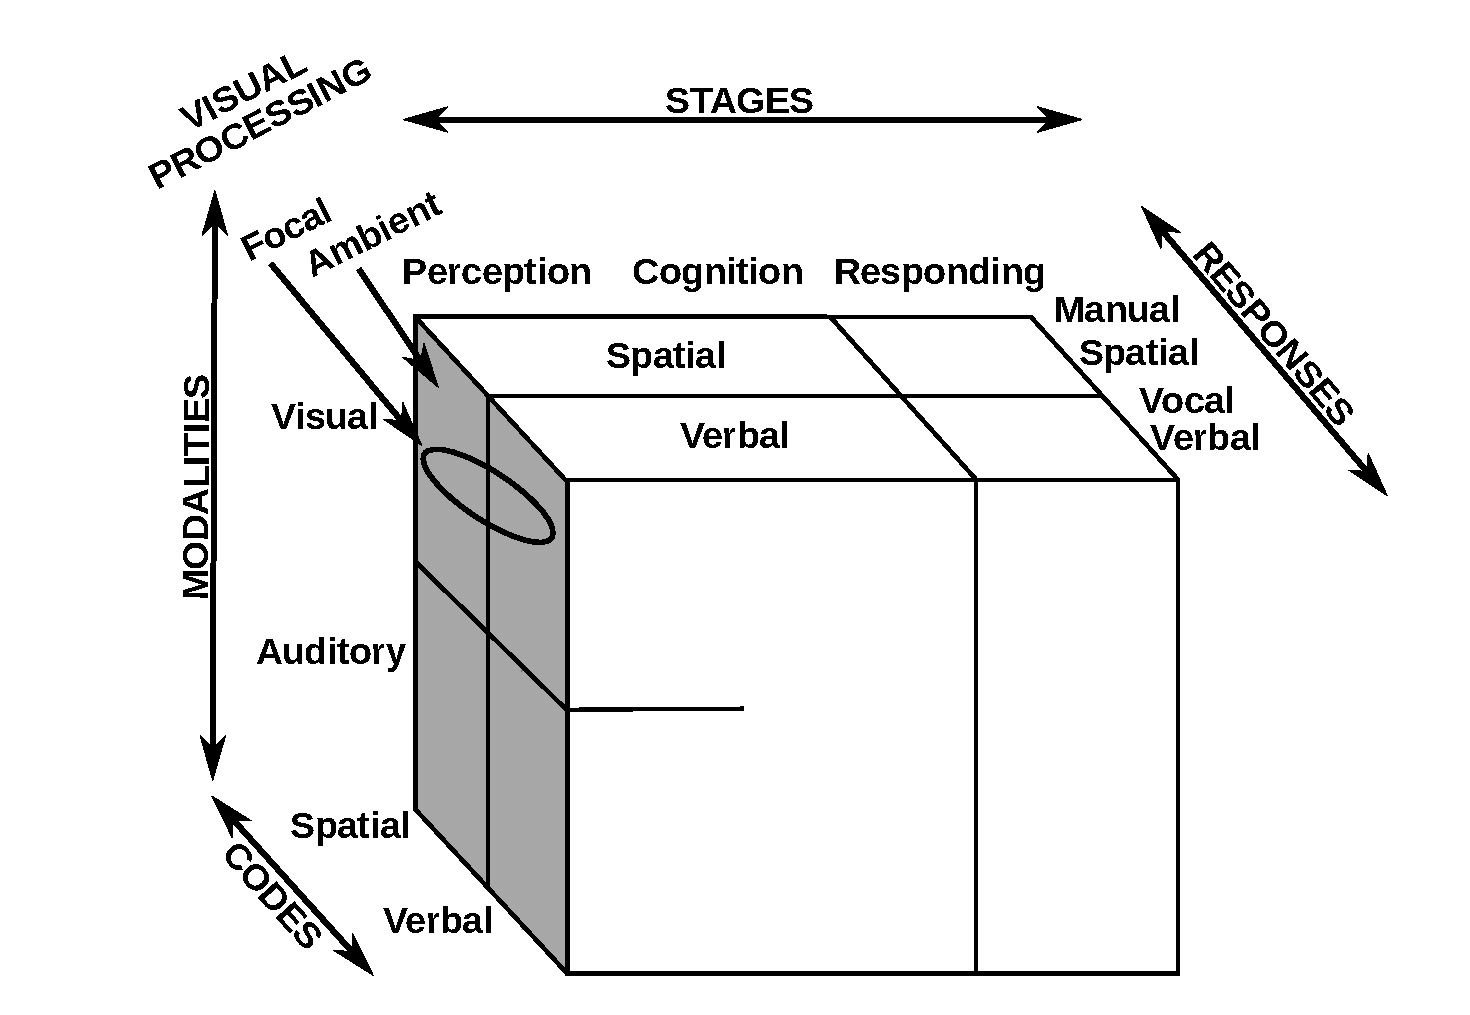
\includegraphics[width=.7\textwidth]{figures/wickenstiescube.pdf}
\caption{Cognitive Load Model (adapted from \citealt[163]{Wickens2002})\label{fig:prandi:1}}
\end{figure}

The result of this adaptation is a Cognitive Resource Footprint (\textsc{crf}), which Seeber (\citeyear{Seeber2007}) also develops for shadowing and sight-translation. Simultaneous interpreting is the combination of two main tasks: the listening and comprehension task on the one hand, and the production and monitoring task on the other. As shown in \figref{fig:prandi:2}, the first task mobilizes auditory-verbal and cognitive-verbal resources at the perceptual-cognitive stage (interpreters receive the aural stimulus, i.e. the words pronounced by the speaker, and analyze the verbal message). The second task requires the same kind of resources at the perceptual-cognitive stage and additional vocal-verbal resources at the response stage (interpreters verbally ``respond'' to what they have heard by delivering the message in the target language, but also listen to and monitor their own rendition).

\begin{figure}
	%%please move the includegraphics inside the {figure} environment
	%%\includegraphics[width=\textwidth]{Ch2-img10.png}
	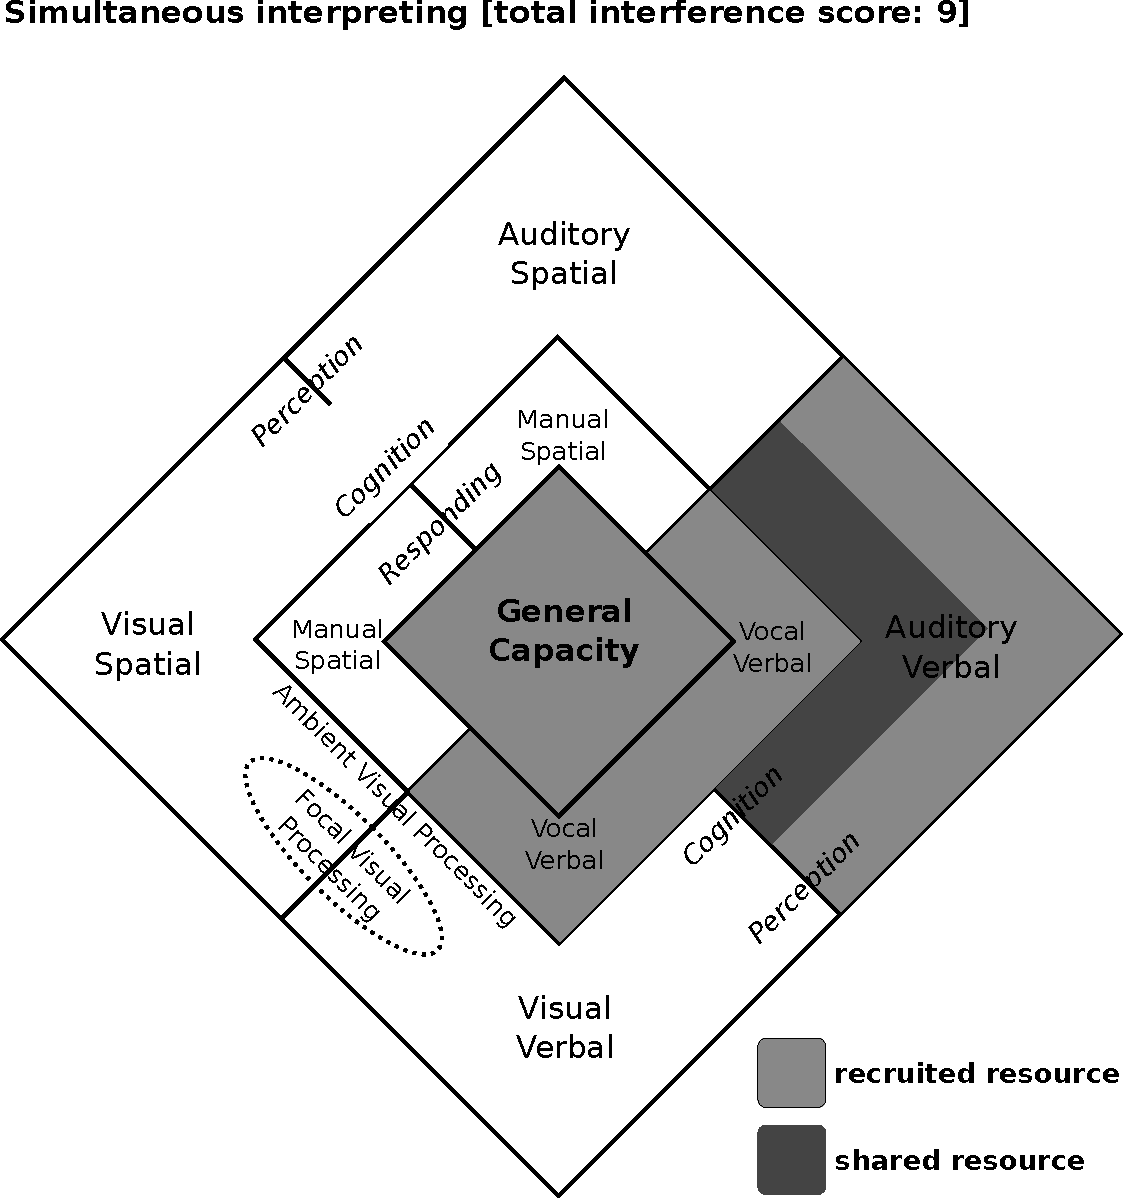
\includegraphics[width=.4\textheight]{figures/Seeberlozenge.pdf}
	\caption{\label{fig:prandi:2}Cognitive resource footprint for simultaneous interpreting (adapted from \citealt[1385]{Seeber2007})}
\end{figure}
 
The footprint is integrated by a Conflict Matrix which shows the degree of interference between two co-occurring tasks as the sum of the demand vectors for each sub-task and of the individual conflict coefficients between sub-tasks (see \figref{fig:prandi:3}). 

The demand vectors indicate the degree to which each sub-task recruits a certain type of resource. Seeber postulates a demand vector of 1 for each sub-task. Conflict coefficients instead show to which degree the single sub-tasks compete for the same resources. When two sub-tasks share resources that are governed by the same structures, their level of conflict is higher than for two sub-tasks that do not share resources (and time-sharing between them is not as efficient). The sum of demand vectors and conflict coefficients produces a value of 9 for simultaneous interpreting.

\begin{figure}[p]
	%%please move the includegraphics inside the {figure} environment
	%%\includegraphics[width=\textwidth]{Ch2-img11.png}
	\resizebox{\textwidth}{!}{\begin{tikzpicture}[
        hea/.style={align=flush center,text width=1.33cm},
        rsma/.style={rotate=90},
        rhea/.style={align=flush center,text width=1.33cm,rotate=90},
        row 1/.style={minimum height=0.665cm},
        row 2/.style={minimum height=0.665cm},
        column 1/.style={minimum width=0.665cm},
        column 2/.style={minimum width=0.665cm},
        ]
\sffamily\footnotesize
\matrix (prandifig3) [matrix of nodes, nodes in empty cells,ampersand replacement=\&] {
\&  \&  \&  \&  \& ~ \&  \&  \&  \&  \&  \&  \\  %\multicolumn{8}{c}{listening \\& comprehension}\\
\&  \&  \&  \&  \& ~ \&  \&  \&  \&  \&  \&  \\  % \multicolumn{4}{c}{perceptual} \& \multicolumn{2}{c}{cognitive} \& \multicolumn{2}{c}{response}\\
\&  \&  \& {vector} \& {$\emptyset$} \& {$\emptyset$} \& {$\emptyset$} \& {1\vphantom{$\emptyset$}} \& {$\emptyset$} \& {1\vphantom{$\emptyset$}} \& {$\emptyset$} \& {$\emptyset$}\\
\&  \& \node[rsma]{demand}; \&  \& \node[hea]{visual\linebreak spatial}; \& \node[hea]{visual\linebreak verbal}; \& \node[hea]{auditory\linebreak spatial}; \& \node[hea] (prandifig3-4-8) {auditory\linebreak verbal}; \& \node[hea]{cognitive\linebreak spatial}; \& \node[hea] (prandifig3-4-10) {cognitive\linebreak verbal}; \& \node[hea]{response\linebreak spatial}; \& \node[hea] (prandifig3-4-12) {response\linebreak verbal}; \\
\&  \& \node[rsma] (prandifig3-5-3) {$\emptyset$}; \& \node[rhea]{visual\linebreak spatial};                       \& {0.8} \& {0.6} \& {0.6} \& {0.4} \& {0.7} \& {0.5} \& {0.4} \& {0.2}\\
\&  \& \node[rsma] (prandifig3-6-3) {$\emptyset$}; \& \node[rhea]{visual\linebreak verbal};                        \& {0.6} \& {0.8} \& {0.4} \& {0.6} \& {0.5} \& {0.7} \& {0.2} \& {0.4}\\
\&  \& \node[rsma] (prandifig3-7-3) {$\emptyset$}; \& \node[rhea]{auditory\linebreak spatial};                     \& {0.6} \& {0.4} \& {0.8} \& {0.4} \& {0.7} \& {0.5} \& {0.4} \& {0.2}\\
\&  \& \node[rsma] (prandifig3-8-3) {1\vphantom{$\emptyset$}};           \& \node[rhea]{auditory\linebreak verbal};    \& {0.4} \& {0.6} \& {0.4} \& {0.8} \& {0.5} \& {0.7} \& {0.2} \& {0.4}\\
\&  \& \node[rsma] (prandifig3-9-3) {$\emptyset$}; \& \node[rhea]{cognitive\linebreak spatial};                    \& {0.7} \& {0.5} \& {0.7} \& {0.5} \& {0.8} \& {0.6} \& {0.6} \& {0.4}\\
\&  \& \node[rsma] (prandifig3-10-3) {1\vphantom{$\emptyset$}};           \& \node[rhea]{cognitive\linebreak verbal};  \& {0.5} \& {0.7} \& {0.5} \& {0.7} \& {0.6} \& {0.8} \& {0.4} \& {0.6}\\
\&  \& \node[rsma] (prandifig3-11-3) {$\emptyset$}; \& \node[rhea]{response\linebreak spatial};                     \& {0.4} \& {0.2} \& {0.4} \& {0.2} \& {0.6} \& {0.4} \& {0.8} \& {0.6}\\
\&  \& \node[rsma] (prandifig3-12-3) {1\vphantom{$\emptyset$}}; \& \node[rhea] (prandifig3-12-4) {response\linebreak verbal};   \& {0.2} \& {0.4} \& {0.2} \& {0.4} \& {0.4} \& {0.6} \& {0.6} \& {1.0}\\
};
\node [fit=(prandifig3-1-5)(prandifig3-1-12)] {listening \& comprehension};
\node [fit=(prandifig3-2-5)(prandifig3-2-8)] {perceptual};
\node [fit=(prandifig3-2-9)(prandifig3-2-10)] {cognitive};
\node [fit=(prandifig3-2-11)(prandifig3-2-12)] {response};
\node [overlay,fit=(prandifig3-5-2)(prandifig3-8-2)  ,rotate=90,text width=2.66cm,inner sep=0pt] {perceptual};
\node [overlay,fit=(prandifig3-9-2)(prandifig3-10-2) ,rotate=90,text width=2.66cm,inner sep=0pt] {cognitive};
\node [overlay,fit=(prandifig3-11-2)(prandifig3-12-2),rotate=90,text width=2.66cm,inner sep=0pt] {response};
\node [overlay,rotate=90,fit=(prandifig3-5-1)(prandifig3-12-1),text width=8cm,inner sep=0pt] {production \& monitoring};
\begin{scope}[on background layer]
\foreach \i in {8,10,12} \node [fit=(prandifig3-\i-3)(prandifig3-\i-12), fill=black!12,minimum height=1.33cm,yshift=-.5ex] {};
\foreach \j in {8,10} \node [fit=(prandifig3-3-\j)(prandifig3-12-\j), fill=black!12,minimum width=1.33cm,inner xsep=0pt] {};
\foreach \x/\y in {8/8,8/10,10/8,10/10,12/8,12/10} \node [fit=(prandifig3-\x-\y), fill=black!50,minimum width=1.33cm,minimum height=1.33cm,yshift=-.75ex] {};
\end{scope}
\draw (prandifig3-4-12.south east) -| (prandifig3-12-4.south west);
\draw (prandifig3-4-12.north east) -| (prandifig3-12-4.north west);
\node (temp32113212) [overlay,fit=(prandifig3-2-11.south west)(prandifig3-2-12.south east),inner ysep=5pt] {}; \draw (temp32113212.north west) -- (temp32113212.north east);
\node (temp3393310) [overlay,fit=(prandifig3-3-9.north west)(prandifig3-3-10.north east),inner ysep=5pt] {};\draw (temp3393310.north west) -- (temp3393310.north east);
\node (temp335338) [overlay,fit=(prandifig3-3-5.north west)(prandifig3-3-8.north east),inner ysep=5pt] {};\draw (temp335338.north west) -- (temp335338.north east);
\node (temp31133123) [overlay,fit=(prandifig3-11-3.north east)(prandifig3-12-3),inner xsep=5pt] {};\draw (temp31133123.north west) -- (temp31133123.south west);
\node (temp3933103) [overlay,fit=(prandifig3-9-3.north east)(prandifig3-10-3),inner xsep=5pt] {};\draw (temp3933103.north west) -- (temp3933103.south west);
\node (temp353383) [overlay,fit=(prandifig3-5-3.north east)(prandifig3-8-3),inner xsep=5pt] {};\draw (temp353383.north west) -- (temp353383.south west);
\end{tikzpicture}
}
\begin{center}\scriptsize
\begin{tabular}{@{}lclcl@{}}
Total interference score & = & demand vectors & + & conflict coefficients\\
                         & = & ($1+1+1+1+1$)    & + & ($0.7+0.8+0.4+0.6+0.8+0.7$)
\end{tabular}
\end{center}
\caption{Conflict matrix for simultaneous interpreting (adapted from \citealt[188]{Seeber2011a})\label{fig:prandi:3}}
\end{figure}

The possibility to ``quantify'' the degree of interference between co-occurring tasks and to explain multi-tasking makes Seeber’s Cognitive Load Model more suited than Gile’s \textsc{em} to formulate hypotheses on simultaneous interpreting with \textsc{cai} tools, as discussed below. For this reason, I chose the Cognitive Load Model for simultaneous interpreting as my theoretical framework.

\subsection{Hypotheses on \textsc{si} with \textsc{cai}}\label{sec:prandi:2.2}\largerpage
Seeber uses his model to represent the allocation of cognitive resources during ``standard'' simultaneous interpreting, without indicating any specific conditions under which this activity is performed. What happens when, during \textsc{si}, the interpreter can query a terminological database? What kind of cognitive resources are recruited, and at which stage? And how much do they interfere with each other?

\begin{figure}[t]
	%%please move the includegraphics inside the {figure} environment
	%%\includegraphics[width=\textwidth]{Ch2-img12.png}
        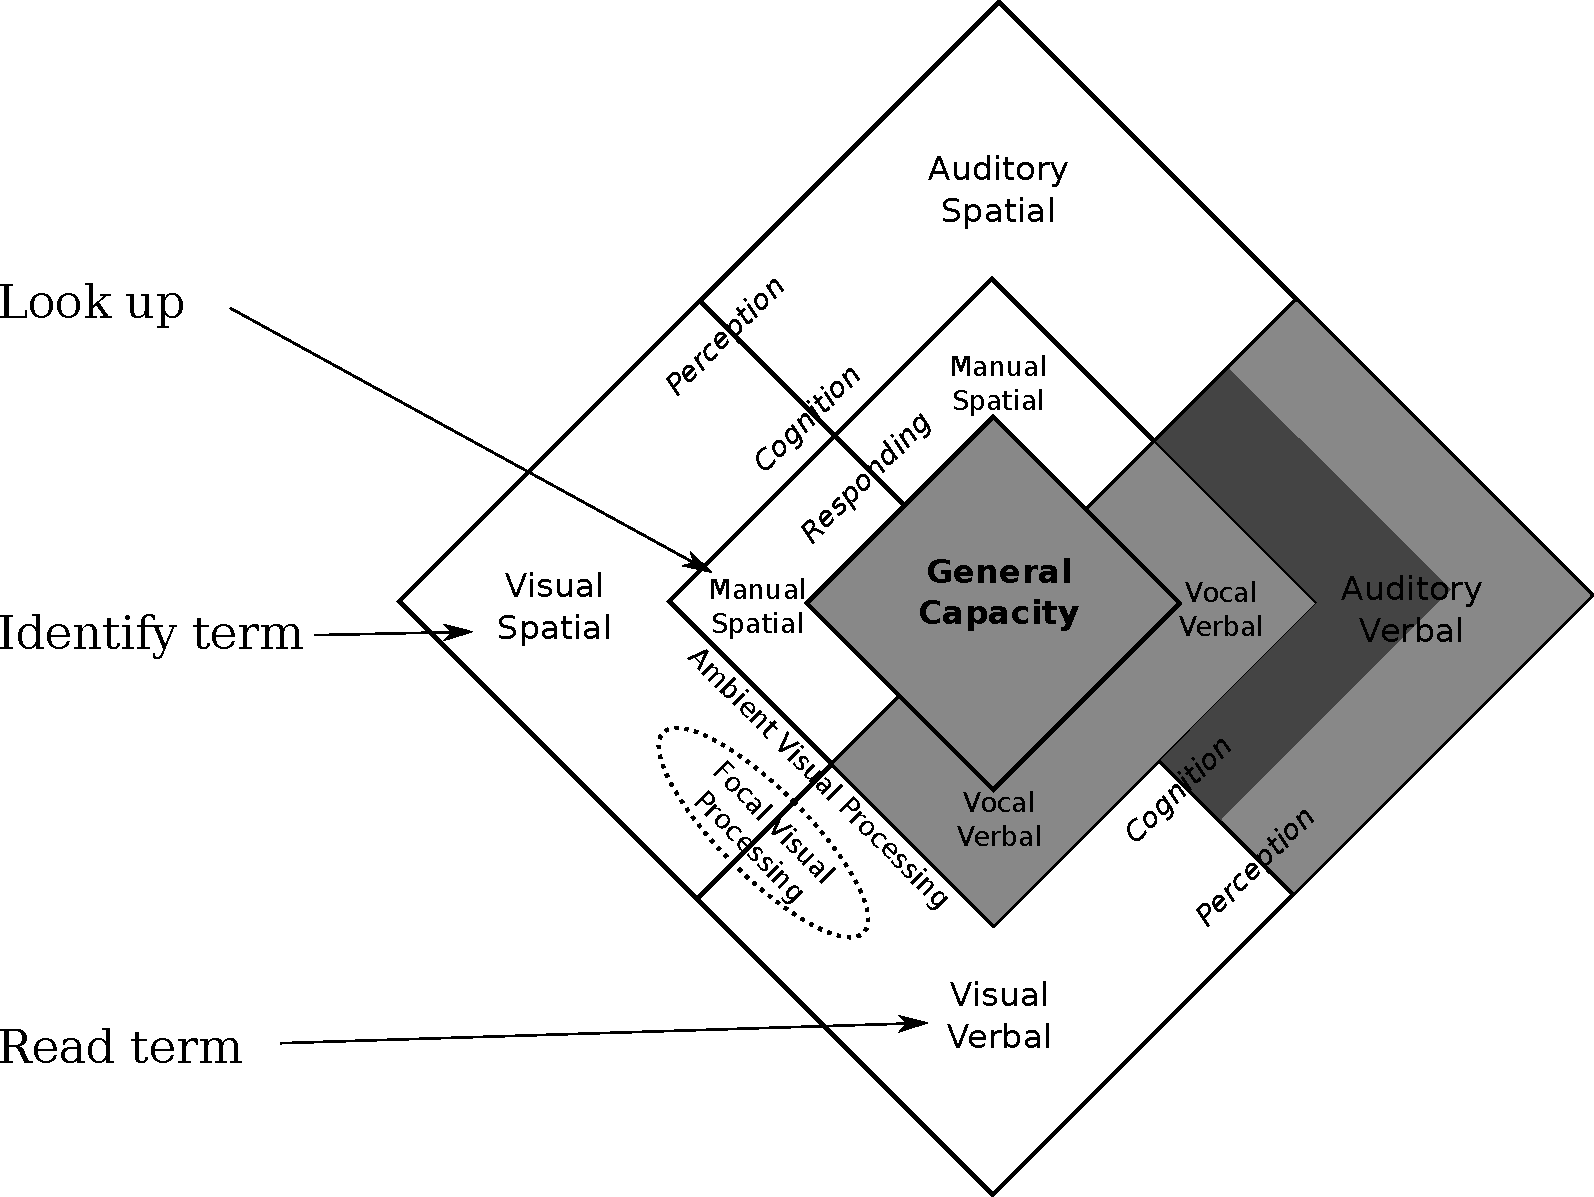
\includegraphics[height=.4\textheight]{figures/fig2-4.pdf}
\caption{Additional cognitive resources recruited during \textsc{si} with a \textsc{cai} tool/electronic glossary\label{fig:prandi:4}}
\end{figure}

In addition to the operations traditionally performed during simultaneous interpreting, when working with a \textsc{cai} tool, or with another terminology management solution -- such as an electronic glossary -- the interpreter has to type a term or part thereof in order to query the database. This action can be considered as a response to the auditory stimulus, a reaction that precedes the vocal-verbal response (i.e. the interpreter’s delivery of the term in question). During the look-up process, manual-spatial resources are therefore recruited at the response stage. After the query has been completed, interpreters are typically presented with a list of terminological pairs (the term and its equivalent(s) in the target language). They will therefore need to visually identify on the screen the term needed, an operation that requires visual-spatial resources at the perceptive-cognitive stage. Once the term has been identified, it is also read, making use of visual-verbal resources in the same stage of the process. As illustrated by Figures~\ref{fig:prandi:4} and \ref{fig:prandi:5}, the Cognitive Resource Footprint for simultaneous interpreting during which a terminological query is performed using a \textsc{cai} tool or an electronic glossary recruits more resources than ``standard'' \textsc{si}. 

\begin{figure}[t]
	%%please move the includegraphics inside the {figure} environment
	%%\includegraphics[width=\textwidth]{Ch2-img13.png}
	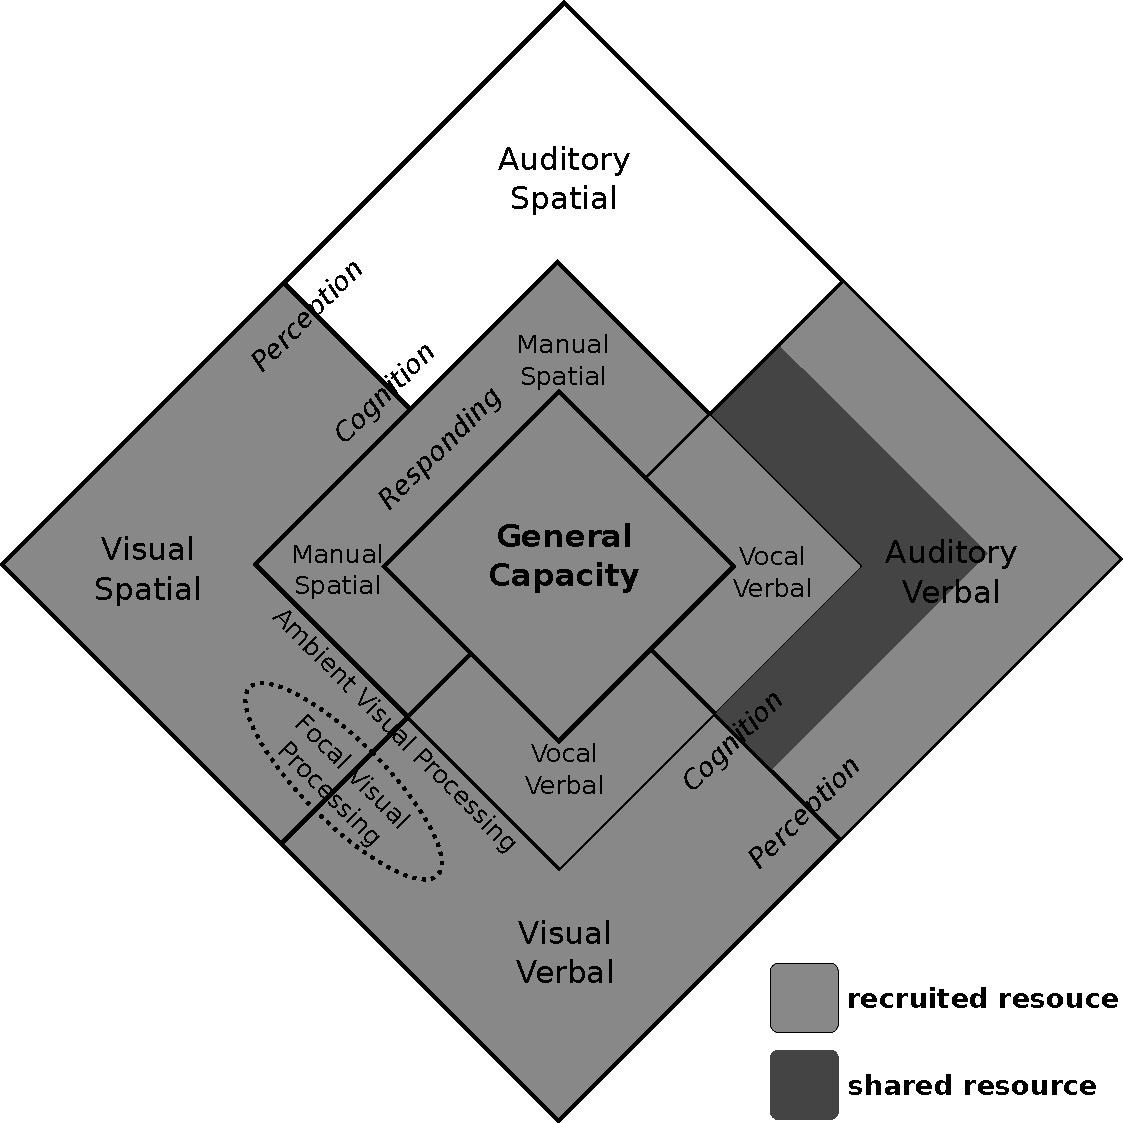
\includegraphics[height=.4\textheight]{figures/fig2-5.pdf}
\caption{\label{fig:prandi:5}Cognitive Resource Footprint for \textsc{si} with a \textsc{cai} tool/electronic glossary}
\end{figure}

It goes without saying that the \textsc{crf} shown in \figref{fig:prandi:5} applies only to those moments when the interpreter is performing a query, and should not be seen as representative of the whole interpreting process. Cognitive load is not static, but rather varies constantly during the interpreting process, as a function of the cognitive resources recruited. I hypothesize that cognitive load is higher while the query is performed, since more cognitive resources are recruited (as shown by the \textsc{crf}). In some cases, it might even lead to cognitive overload. If the term retrieval is successful, however, I expect cognitive load to go back to normal levels during production. Cognitive load might even be lower than for ``standard'' simultaneous interpreting, as the search for the appropriate term in the interpreter’s memory would be replaced by a query in the glossary.

\begin{figure}[p]
	%%please move the includegraphics inside the {figure} environment
	%%\includegraphics[width=\textwidth]{Ch2-img14.png}
\resizebox{\textwidth}{!}{\begin{tikzpicture}[
        hea/.style={align=flush center,text width=1.33cm},
        rsma/.style={rotate=90},
        rhea/.style={align=flush center,text width=1.33cm,rotate=90},
        row 1/.style={minimum height=0.665cm},
        row 2/.style={minimum height=0.665cm},
        column 1/.style={minimum width=0.665cm},
        column 2/.style={minimum width=0.665cm},
        ]
\sffamily\footnotesize
\matrix (prandifig7) [matrix of nodes, nodes in empty cells,ampersand replacement=\&] {
\&  \&  \&  \&  \& ~ \&  \&  \&  \&  \&  \&  \\  %\multicolumn{8}{c}{listening \\& comprehension}\\
\&  \&  \&  \&  \& ~ \&  \&  \&  \&  \&  \&  \\  % \multicolumn{4}{c}{perceptual} \& \multicolumn{2}{c}{cognitive} \& \multicolumn{2}{c}{response}\\
\&  \&  \& {vector} \& {$\emptyset$} \& {$\emptyset$} \& {$\emptyset$} \& {1\vphantom{$\emptyset$}} \& {$\emptyset$} \& {1\vphantom{$\emptyset$}} \& {$\emptyset$} \& \node [hea] (prandifig7-3-12) {$\emptyset$};\\
\&  \& \node[rsma]{demand}; \&  \& \node[hea]{visual\linebreak spatial}; \& \node[hea]{visual\linebreak verbal}; \& \node[hea]{auditory\linebreak spatial}; \& \node[hea] (prandifig7-4-8) {auditory\linebreak verbal}; \& \node[hea]{cognitive\linebreak spatial}; \& \node[hea] (prandifig7-4-10) {cognitive\linebreak verbal}; \& \node[hea]{response\linebreak spatial}; \& \node[hea] (prandifig7-4-12) {response\linebreak verbal}; \\
\&  \& \node[rsma] (prandifig7-5-3) {2\vphantom{$\emptyset$}}; \& \node[rhea]{visual\linebreak spatial};    \& {0.8} \& {0.6} \& {0.6} \& {0.4} \& {0.7} \& {0.5} \& {0.4} \& 0.2\\
\&  \& \node[rsma] (prandifig7-6-3) {2\vphantom{$\emptyset$}}; \& \node[rhea]{visual\linebreak verbal};     \& {0.6} \& {0.8} \& {0.4} \& {0.6} \& {0.5} \& {0.7} \& {0.2} \& {0.4}\\
\&  \& \node[rsma] (prandifig7-7-3) {$\emptyset$}; \& \node[rhea]{auditory\linebreak spatial};  \& {0.6} \& {0.4} \& {0.8} \& {0.4} \& {0.7} \& {0.5} \& {0.4} \& {0.2}\\
\&  \& \node[rsma] (prandifig7-8-3) {1\vphantom{$\emptyset$}};           \& \node[rhea]{auditory\linebreak verbal};   \& {0.4} \& {0.6} \& {0.4} \& {0.8} \& {0.5} \& {0.7} \& {0.2} \& {0.4}\\
\&  \& \node[rsma] (prandifig7-9-3) {$\emptyset$}; \& \node[rhea]{cognitive\linebreak spatial}; \& {0.7} \& {0.5} \& {0.7} \& {0.5} \& {0.8} \& {0.6} \& {0.6} \& {0.4}\\
\&  \& \node[rsma] (prandifig7-10-3) {1\vphantom{$\emptyset$}};           \& \node[rhea]{cognitive\linebreak verbal};  \& {0.5} \& {0.7} \& {0.5} \& {0.7} \& {0.6} \& {0.8} \& {0.4} \& {0.6}\\
\&  \& \node[rsma] (prandifig7-11-3) {2\vphantom{$\emptyset$}}; \& \node[rhea]{response\linebreak spatial};  \& {0.4} \& {0.2} \& {0.4} \& {0.2} \& {0.6} \& {0.4} \& {0.8} \& {0.6}\\
\&  \& \node[rsma] (prandifig7-12-3) {1\vphantom{$\emptyset$}}; \& \node[rhea] (prandifig7-12-4) {response\linebreak verbal};   \& {0.2} \& {0.4} \& {0.2} \& {0.4} \& {0.4} \& {0.6} \& {0.6} \& {1.0}\\
};
\node [fit=(prandifig7-1-5)(prandifig7-1-12)] {listening \& comprehension};
\node [fit=(prandifig7-2-5)(prandifig7-2-8)] {perceptual};
\node [fit=(prandifig7-2-9)(prandifig7-2-10)] {cognitive};
\node [fit=(prandifig7-2-11)(prandifig7-2-12)] {response};
\node [overlay,fit=(prandifig7-5-2)(prandifig7-8-2)  ,rotate=90,text width=2.66cm,inner sep=0pt] {perceptual};
\node [overlay,fit=(prandifig7-9-2)(prandifig7-10-2) ,rotate=90,text width=2.66cm,inner sep=0pt] {cognitive};
\node [overlay,fit=(prandifig7-11-2)(prandifig7-12-2),rotate=90,text width=2.66cm,inner sep=0pt] {response};
\node [overlay,rotate=90,fit=(prandifig7-5-1)(prandifig7-12-1),text width=8cm,inner sep=0pt] {production \& monitoring};
\begin{scope}[on background layer]
\foreach \i in {5,6,8,10,11,12} \node [fit=(prandifig7-\i-3)(prandifig7-\i-12),fill=black!12,minimum height=1.33cm,yshift=-.5ex] {};
\foreach \j in {8,10} \node [fit=(prandifig7-3-\j)(prandifig7-12-\j), fill=black!12,minimum width=1.33cm,inner xsep=0pt] {};
\foreach \x/\y in {5/8,5/10,6/8,6/10,8/8,8/10,10/8,10/10,11/8,11/10,12/8,12/10} {\node [fit=(prandifig7-\x-\y), fill=black!50,minimum width=1.33cm,minimum height=1.33cm,yshift=-.75ex] {};}
\end{scope}
\draw (prandifig7-4-12.south east) -| (prandifig7-12-4.south west);
\draw (prandifig7-4-12.north east) -| (prandifig7-12-4.north west);
\node (temp32113212) [overlay,fit=(prandifig7-2-11.south west)(prandifig7-2-12.south east),inner ysep=5pt] {}; \draw (temp32113212.north west) -- (temp32113212.north east);
\node (temp3393310) [overlay,fit=(prandifig7-3-9.north west)(prandifig7-3-10.north east),inner ysep=5pt] {};\draw (temp3393310.north west) -- (temp3393310.north east);
\node (temp335338) [overlay,fit=(prandifig7-3-5.north west)(prandifig7-3-8.north east),inner ysep=5pt] {};\draw (temp335338.north west) -- (temp335338.north east);
\node (temp31133123) [overlay,fit=(prandifig7-11-3.north east)(prandifig7-12-3),inner xsep=5pt] {};\draw (temp31133123.north west) -- (temp31133123.south west);
\node (temp3933103) [overlay,fit=(prandifig7-9-3.north east)(prandifig7-10-3),inner xsep=5pt] {};\draw (temp3933103.north west) -- (temp3933103.south west);
\node (temp353383) [overlay,fit=(prandifig7-5-3.north east)(prandifig7-8-3),inner xsep=5pt] {};\draw (temp353383.north west) -- (temp353383.south west);
\end{tikzpicture}}
\caption{Conflict matrix for \textsc{si} with spreadsheet (Excel) TIC = 16.8\label{fig:prandi:6}}
\end{figure}

\begin{figure}[p]
	%%please move the includegraphics inside the {figure} environment
	%%\includegraphics[width=\textwidth]{Ch2-img15.png}
\resizebox{\textwidth}{!}{\begin{tikzpicture}[
        hea/.style={align=flush center,text width=1.33cm},
        rsma/.style={rotate=90},
        rhea/.style={align=flush center,text width=1.33cm,rotate=90},
        row 1/.style={minimum height=0.665cm},
        row 2/.style={minimum height=0.665cm},
        column 1/.style={minimum width=0.665cm},
        column 2/.style={minimum width=0.665cm},
        ]
\sffamily\footnotesize
\matrix (prandifig6) [matrix of nodes, nodes in empty cells,ampersand replacement=\&] {
\&  \&  \&  \&  \& ~ \&  \&  \&  \&  \&  \&  \\  %\multicolumn{8}{c}{listening \\& comprehension}\\
\&  \&  \&  \&  \& ~ \&  \&  \&  \&  \&  \&  \\  % \multicolumn{4}{c}{perceptual} \& \multicolumn{2}{c}{cognitive} \& \multicolumn{2}{c}{response}\\
\&  \&  \& {vector} \& {$\emptyset$} \& {$\emptyset$} \& {$\emptyset$} \& {1\vphantom{$\emptyset$}} \& {$\emptyset$} \& {1\vphantom{$\emptyset$}} \& {$\emptyset$} \& {$\emptyset$}\\
\&  \& \node[rsma]{demand}; \&  \& \node[hea]{visual\linebreak spatial}; \& \node[hea]{visual\linebreak verbal}; \& \node[hea]{auditory\linebreak spatial}; \& \node[hea] (prandifig6-4-8) {auditory\linebreak verbal}; \& \node[hea]{cognitive\linebreak spatial}; \& \node[hea] (prandifig6-4-10) {cognitive\linebreak verbal}; \& \node[hea]{response\linebreak spatial}; \& \node[hea] (prandifig6-4-12) {response\linebreak verbal}; \\
\&  \& \node[rsma] (prandifig6-5-3) {2\vphantom{$\emptyset$}}; \& \node[rhea]{visual\linebreak spatial};                       \& {0.8} \& {0.6} \& {0.6} \& {0.4} \& {0.7} \& {0.5} \& {0.4} \& {0.2}\\
\&  \& \node[rsma] (prandifig6-6-3) {2\vphantom{$\emptyset$}}; \& \node[rhea]{visual\linebreak verbal};                        \& {0.6} \& {0.8} \& {0.4} \& {0.6} \& {0.5} \& {0.7} \& {0.2} \& {0.4}\\
\&  \& \node[rsma] (prandifig6-7-3) {$\emptyset$}; \& \node[rhea]{auditory\linebreak spatial};                     \& {0.6} \& {0.4} \& {0.8} \& {0.4} \& {0.7} \& {0.5} \& {0.4} \& {0.2}\\
\&  \& \node[rsma] (prandifig6-8-3) {\vphantom{$\emptyset$}1};           \& \node[rhea]{auditory\linebreak verbal};    \& {0.4} \& {0.6} \& {0.4} \& {0.8} \& {0.5} \& {0.7} \& {0.2} \& {0.4}\\
\&  \& \node[rsma] (prandifig6-9-3) {$\emptyset$}; \& \node[rhea]{cognitive\linebreak spatial};                    \& {0.7} \& {0.5} \& {0.7} \& {0.5} \& {0.8} \& {0.6} \& {0.6} \& {0.4}\\
\&  \& \node[rsma] (prandifig6-10-3) {\vphantom{$\emptyset$}1};           \& \node[rhea]{cognitive\linebreak verbal};  \& {0.5} \& {0.7} \& {0.5} \& {0.7} \& {0.6} \& {0.8} \& {0.4} \& {0.6}\\
\&  \& \node[rsma] (prandifig6-11-3) {2\vphantom{$\emptyset$}}; \& \node[rhea]{response\linebreak spatial};                     \& {0.4} \& {0.2} \& {0.4} \& {0.2} \& {0.6} \& {0.4} \& {0.8} \& {0.6}\\
\&  \& \node[rsma] (prandifig6-12-3) {1\vphantom{$\emptyset$}};           \& \node[rhea] (prandifig6-12-4) {response\linebreak verbal};   \& {0.2} \& {0.4} \& {0.2} \& {0.4} \& {0.4} \& {0.6} \& {0.6} \& {1.0}\\
};
\node [fit=(prandifig6-1-5)(prandifig6-1-12)] {listening \& comprehension};
\node [fit=(prandifig6-2-5)(prandifig6-2-8)] {perceptual};
\node [fit=(prandifig6-2-9)(prandifig6-2-10)] {cognitive};
\node [fit=(prandifig6-2-11)(prandifig6-2-12)] {response};
\node [overlay,fit=(prandifig6-5-2)(prandifig6-8-2)  ,rotate=90,text width=2.66cm,inner sep=0pt] {perceptual};
\node [overlay,fit=(prandifig6-9-2)(prandifig6-10-2) ,rotate=90,text width=2.66cm,inner sep=0pt] {cognitive};
\node [overlay,fit=(prandifig6-11-2)(prandifig6-12-2),rotate=90,text width=2.66cm,inner sep=0pt] {response};
\node [overlay,rotate=90,fit=(prandifig6-5-1)(prandifig6-12-1),text width=8cm,inner sep=0pt] {production \& monitoring};
\begin{scope}[on background layer]
\foreach \i in {5,6,8,10,11,12} \node [fit=(prandifig7-\i-3)(prandifig7-\i-12), fill=black!12,minimum height=1.33cm,yshift=-.5ex,inner ysep=0pt] {};
\foreach \j in {8,10} \node [fit=(prandifig7-3-\j)(prandifig7-12-\j), fill=black!12,minimum width=1.33cm,inner xsep=0pt] {};
\foreach \x in {5,6,8,10,11,12} {
    \foreach \y in {8,10} \node [fit=(prandifig7-\x-\y), fill=black!50,minimum width=1.33cm,minimum height=1.33cm,yshift=-.75ex] {};
    }
\end{scope}
\draw (prandifig6-4-12.south east) -| (prandifig6-12-4.south west);
\draw (prandifig6-4-12.north east) -| (prandifig6-12-4.north west);
\node (temp32113212) [overlay,fit=(prandifig6-2-11.south west)(prandifig6-2-12.south east),inner ysep=5pt] {}; \draw (temp32113212.north west) -- (temp32113212.north east);
\node (temp3393310) [overlay,fit=(prandifig6-3-9.north west)(prandifig6-3-10.north east),inner ysep=5pt] {};\draw (temp3393310.north west) -- (temp3393310.north east);
\node (temp335338) [overlay,fit=(prandifig6-3-5.north west)(prandifig6-3-8.north east),inner ysep=5pt] {};\draw (temp335338.north west) -- (temp335338.north east);
\node (temp31133123) [overlay,fit=(prandifig6-11-3.north east)(prandifig6-12-3),inner xsep=5pt] {};\draw (temp31133123.north west) -- (temp31133123.south west);
\node (temp3933103) [overlay,fit=(prandifig6-9-3.north east)(prandifig6-10-3),inner xsep=5pt] {};\draw (temp3933103.north west) -- (temp3933103.south west);
\node (temp353383) [overlay,fit=(prandifig6-5-3.north east)(prandifig6-8-3),inner xsep=5pt] {};\draw (temp353383.north west) -- (temp353383.south west);
\end{tikzpicture}}
\caption{Conflict matrix for \textsc{si} with \textsc{cai} (InterpretBank) TIC = 14.8\label{fig:prandi:7}}
\end{figure}


If one only took into consideration the Cognitive Resource Footprint, one would not, however, be able to formulate hypotheses on the differences in Cognitive Load experienced while working with a \textsc{cai} tool or with less advanced terminology management solutions, such as electronic glossaries in the form of a Word or Excel table. These differences can be explored by assigning a different demand vector to the various terminology management solutions. The Conflict Matrices can thus help visually represent the different levels of recruitment of cognitive resources. If the glossary is the same, what varies among the tools are the user interface and the search algorithm. The most advanced \textsc{cai} tools, and InterpretBank\footnote{\url{http://www.interpretbank.com}} in particular, which I adopt in the study, are designed to yield the most accurate results and to facilitate the user in identifying the term needed on the screen. I therefore expect the tools to require a lower level of manual-spatial resources (to look up the term) and of visual-spatial resources (to locate the term on the screen), when compared, for instance, to an Excel spreadsheet. As shown in Figures~\ref{fig:prandi:6} and~\ref{fig:prandi:7}, I can therefore assign a demand vector of 1 to each of these resources in the case of \textsc{cai} tools, and a demand vector of 2 in the case of an Excel spreadsheet. The total interference score for \textsc{si} performed during the use of a \textsc{cai} tool would therefore be equal to 14.8, while for \textsc{si} with the use of an Excel spreadsheet it would be higher (16.8).

The integration of automatic speech recognition in a \textsc{cai} tool (see \citealp{Fantinuoli2017b}) would require no manual-spatial resources, thus lowering the total interference score to at least 13.2.

\section{Designing a pilot study on the use of \textsc{cai} tools in the booth}\label{sec:prandi:3}
\subsection{Introduction}\label{sec:prandi:3.1}
The debate around how \textsc{cai} tools influence the process and the quality of interpretation is in large measure not based on empirical data, which are still very scarce and limited to a few small experiments, but is rather the result of personal beliefs and assumptions which have not been proven empirically. A research project currently underway at the University of Mainz\slash Germersheim \citep{Prandi2016, Prandi2017a, Prandi2017b} aims at bridging this research gap by providing data that can substantiate arguments in favor and against \textsc{cai} tools. One source of difficulty in the investigation of \textsc{cai} tools lies in the fact that no research methodology for the combined collection of data both on the process and on the product of \textsc{si} with \textsc{cai} has been developed and tested yet. In order to provide a first solution to this issue, I therefore conducted an exploratory study with the aim of evaluating the appropriateness of the stimuli used for data collection. In the following sections I will present my research questions, describe the structure of the exploratory study and illustrate the stimuli used. The analysis of the participants’ renditions is the subject of the remainder of the chapter.

\subsection{Research questions}\label{sec:prandi:3.2}
My research project aims at answering three fundamental questions:

\begin{itemize}
\item Do \textsc{cai} tools help improve the terminological quality of the interpretation when compared to traditional electronic glossaries?
\item Does a query performed with a \textsc{cai} tool during \textsc{si} lead to lower additional local cognitive load when compared to traditional glossary prepared with Word or Excel? Does looking up terminology lead to cognitive overload and if so, does this also happen when \textsc{cai} tools are used?
\item Can a combination of eye-tracking measures, key-logging data and transcription analysis be used to acquire data on the interpreting process, the terminological quality of the product and the usability of \textsc{cai} tools?
\end{itemize}

In order to first collect data to help answer these questions, an exploratory study was conducted between May and July 2017 at the University of Mainz\slash Germersheim. For the scope of this paper, I will report on the observations made during the analysis of the product, while further work will be required to address the issues related to the process of simultaneous interpreting with \textsc{cai} tools.

\subsection{Structure of the study: sample, duration, training and data collection}\label{sec:prandi:3.3}
The pilot study involved 6 advanced students of the Master’s degree in conference interpreting of the University of Mainz\slash Germersheim. Prior to the study, all students had had at least 3 semesters of practice in simultaneous and consecutive interpreting and had English in their combination as a B or C language. Half of the sample was made up of German natives (one male and two females), half of Italian natives (one female and two males). The test subjects were recruited by e-mail and their participation in the experiment was voluntary. No monetary compensation was offered, but the participation in the study gave the trainees the opportunity to learn about a new tool, InterpretBank, and to practice in the booth with a laptop, something they rarely do systematically in class.

The trainees attended one preliminary meeting which covered the basics of terminology management for conference interpreters. The presentation was centered on practice rather than theory, since a previous study confirmed this was more beneficial to achieve a good level of expertise \citep{Prandi2015a, Prandi2015b}. The search functions in Word, Excel and InterpretBank were described in detail. For the purpose of the study, participants could visualize all the results of a query when working with Word\footnote{The results are displayed in a column on the left-hand side of the window.}, while they had to move to the next occurrence when using Excel. In the presentation I made sure to adopt a neutral approach to the different tools, so as not to favor the \textsc{cai} tool chosen.

After covering the basics, 5 practice sessions followed in the subsequent weeks, with around 1 session per week. During each training session, the students interpreted 3 short speeches from English into their mother tongue (either German or Italian). They could use a glossary provided by the author, for both language combinations, which they could access in all three formats (Word, Excel or InterpretBank). During each session, they used a different tool for each speech, so equal practice time was dedicated to each tool. The first few speeches had been prepared ad-hoc by the author for a previous study \citep{Prandi2015a, Prandi2015b}, while the last few speeches were authentic speeches selected by the author, so as to ensure a certain progression in the practice material. The topics covered during the practice sessions were medicine and biology. After the last session, the students took a short test to verify their proficiency in the use of the tools. All students passed the test and were deemed ready for data collection.

Data collection took place in the \textit{Translation and Cognition Centre} of the University of Mainz\slash Germersheim. The test subjects were briefed about the structure of the study and were informed that they were going to interpret 3 speeches from English into their mother tongue. They were told the topic of the speeches (renewables and other sources of energy) right before data collection started. While this does not reflect professional practice, which requires thorough preparation before interpretation proper, the students were not given the chance to prepare in advance since this would have introduced an additional variable in the study. The methods of preparation and the time dedicated to this fundamental phase of interpreting are very personal and would have been very difficult to standardize and to verify. I therefore decided to sacrifice some ecological validity to limit the number of independent variables.

Every test subject interpreted 3 speeches, each about 12 minutes long and with an average speed of 122.26 words per minute. This speed was chosen to make sure that looking up terminology during interpreting was challenging, but not impossible. All three speeches had been prepared ad-hoc for the study and previously recorded by a native speaker of British English. One glossary of 421 terms was prepared by the author. It contained the same terms for both language combinations and had a simple tabular structure – one column for the source language and one for the target language. The glossary was prepared with InterpretBank and then exported as an Excel spreadsheet, which was then also converted into a Word table. The glossaries were not shown to the test subjects before the interpreting task started. During the interpreting task, the screen was divided in two areas. On the left-hand side, the test subjects could see the video of the speaker, which served as a fixation cross when no term query was being performed. The glossary window was placed on the right-hand side of the screen.

The test subjects’ deliveries were recorded with Audacity, while an \textsc{smi\linebreak red250m} eye-tracker was used to record eye movements. A \textsc{log} file, automatically created by InterpretBank, served as a reference to check what terms had been looked up by the test subjects. The same was done manually for the trials in which Word and Excel were adopted, using the Gaze Replay recordings. The interpretations were then transcribed using Partitur Editor, the transcription tool of the Exmaralda suite, and then analyzed. Before presenting the method used for this analysis and its results in \sectref{sec:prandi:5}, I will describe the main features of the speeches used for data collection, with a focus on stimuli distribution and morphological complexity.

\section{Stimuli features and distribution}\label{sec:prandi:4}
While asking the test subjects to interpret single terms would have eliminated the time constraint typical of simultaneous interpreting, working with authentic, unedited speeches would have introduced too many variables in the experiment. For this reason, I decided to adapt \citeauthor{Seeber2011a}’s methodology (\citeyear{Seeber2011a}) by creating ad-hoc speeches made up of sentence clusters. This method presents three main advantages. First, it enables me to focus the investigation on the target sentences (i.e. the ones which include the stimulus). Second, it makes it easier to work with comparable speeches, as they have the same structure. Third, it gives the test subjects the impression that they are interpreting a speech, rather than disconnected sentences, thus helping me retain a certain degree of ecological validity. Each sentence cluster is composed of a general, introductory sentence, followed by the target sentence containing the stimulus, followed by a third sentence which, like the first one, does not contain specialized terminology. The structure is repeated throughout the speech, so that each stimulus is separated from the next one by two sentences. Here is an example from speech no. 1:

\ea
So we need to change this basic trend and this is why the urgency is there.

In our policies, we should definitely address the need to improve \textbf{vehicle efficiency}.

But there is still much more we can do, in many other areas, as you are aware.

At the \textsc{eu} level, there is another policy option that can help us.

By focusing, for instance, on \textbf{woody biomass fuels}, we can truly make a difference.

They have the potential to help us respond to the challenges we’re facing.
\z

Each speech prepared for data collection contained 36 terms, 12 of which are unigrams (e.g. ``bioenergy''), 12 bigrams (e.g. ``energy poverty'') and 12 trigrams (e.g. ``pressurized water reactor''). This variable was introduced because the structure of the stimuli is expected to also play a role in the usability of the tools. I expect there to be differences between tools when a more morphologically complex term is looked up – it should be more difficult to find a trigram when using a Word or an Excel glossary than when working with a \textsc{cai} tool. 

Of each group of stimuli, 6 are placed at the end of the sentence and 6 in the middle of the sentence. This was done to verify whether the stimulus position has an impact on cognitive load and on the test subjects’ behavior in querying the glossary. I expect the stimuli placed at the end of the sentence to lead to a lower increase in cognitive load and to be looked up more often, thanks to anticipation. 

Of the 6 terms placed at the end of the sentence, 3 should require a query in the glossary, because they are less frequent and thus probably unknown to the participants, and 3 should not.\footnote{This classification was based on the frequency of the terms as per the 2015 news corpus, the 2012 web corpus (\textsc{uk}) and the 2016 Wikipedia corpus for the English language (Projekt Deutscher Wortschatz, \url{http://wortschatz.uni-leipzig.de}).} The same is true for the terms placed in the middle of the sentence. Half of the stimuli in each speech should therefore require a query and half should not. This variable was introduced to verify whether \textsc{cai} tools, which are usually deemed to be user-friendlier and to take up fewer cognitive resources, allow participants to perform more queries without leading to a higher number of errors or omissions. \figref{fig:prandi:8} sums up the features of the stimuli and their distribution in each speech. For each speech, the stimuli can thus be classified according to their features, for future analysis. \tabref{tab:prandi:1} shows an example of this classification for the stimuli in speech nr. 1.

\begin{figure}
\footnotesize
		%%please move the includegraphics inside the {figure} environment
		%%\includegraphics[width=\textwidth]{Ch2-img16.png}
\begin{forest}for tree={grow=east,edge=-{Stealth[]},parent anchor=east,anchor=west}
[36 terms\slash speech
    [12 1-grams
        [6 end sentence,tier=sub
            [3 querying needed,tier=word]
            [3 querying not needed,tier=word]
        ]
        [6 middle sentence,tier=sub
            [3 querying needed,tier=word]
            [3 querying not needed,tier=word]
        ]
    ]
    [12 2-grams
        [6 end sentence,tier=sub
            [3 querying needed,tier=word]
            [3 querying not needed,tier=word]
        ]
        [6 middle sentence,tier=sub
            [3 querying needed,tier=word]
            [3 querying not needed,tier=word]
        ]
    ]    
    [12 3-grams
        [6 end sentence,tier=sub
            [3 querying needed,tier=word]
            [3 querying not needed,tier=word]
        ]
        [6 middle sentence,tier=sub
            [3 querying needed,tier=word]
            [3 querying not needed,tier=word]
        ]
    ]
]
\end{forest}
\caption{Features and distribution of the stimuli used for data collection\label{fig:prandi:8}}
\end{figure}

 

\begin{table}\footnotesize
	\caption{Stimuli classification -- speech 1\label{tab:prandi:1}}
\begin{tabularx}{\linewidth}{Xccc}
\lsptoprule
{Stimulus} & {Position} & {Morphological} & {Glossary search}\\
		   &            &  complexity      & needed (GS)\\\midrule
bioenergy & E & 1 & \\
security of supply & M & 3 & \\
gasoline & M & 1 & \\
conventional fossil fuels & M & 3 & \\
vehicle efficiency & E & 2 & X\\
woody biomass fuels & M & 3 & X\\
liquid biofuels & E & 2 & \\
rapeseed methyl ester & E & 3 & X\\
transesterification & E & 1 & X\\
short-rotation coppice & E & 3 & X\\
black liquor & E & 2 & X\\
corn stover & E & 2 & X\\
lignocellulosic solid biomass & E & 3 & X\\
gasification & M & 1 & X\\
gasifier & E & 1 & \\
green charcoal & M & 2 & X\\
briquettes & M & 1 & X\\
biofuels sector & M & 2 & \\
soil protection & E & 2 & \\
petroleum & M & 1 & \\
greenhouse gas emissions & E & 3 & \\
EU biofuels directive & M & 3 & X\\
indicative targets & M & 2 & X\\
incentives & E & 1 & \\
set-aside land & M & 3 & X\\
arable land & M & 2 & \\
solar power & M & 2 & \\
second-generation biofuels & E & 3 & \\
switchgrass & E & 1 & X\\
first-generation biofuels & E & 3 & \\
residue cake & M & 2 & X\\
milling & E & 1 & X\\
malting & M & 1 & X\\
overall energy demand & M & 3 & \\
renewables & M & 1 & \\
energy mix & E & 2 & \\
\lspbottomrule
\end{tabularx}
\end{table}

\section{Stimuli validation}\label{sec:prandi:5}
One of the aims of the exploratory study was to verify whether the stimuli prepared for data collection, to be also used in a future experiment involving a larger sample, elicited the reaction I expected from the test subjects, i.e. a query in the glossary. This is necessary to make sure that enough queries are performed in the glossary to provide sufficient data for a comparison between the three terminology management solutions I focus my analysis on – Word glossaries, Excel glossaries and second-generation \textsc{cai} tools. While a certain degree of inter-subject variability can be expected, I must verify whether my a-priori classification of the stimuli holds true on a general level. This is the focus of the first part of the transcription analysis which will be presented in \sectref{sec:prandi:5.1}.

Another goal of my research is to verify whether the use of a \textsc{cai} tool leads to better terminological quality in comparison to more traditional terminology management solutions, e.g. Word and Excel glossaries. First observations made in the sample are briefly discussed in \sectref{sec:prandi:5.2}, where I also provide a framework to analyze errors and omissions in relation to the tools used for glossary query.

\sectref{sec:prandi:5.3}
presents the results of my observations in relation to the strategies adopt\-ed by the test subjects to interpret the stimuli. Given the small size of the sample, with this exploratory study I aim to develop a methodology to be used for further research, rather than to draw conclusions, which will require a larger data set. 

\subsection{Stimuli classification}\label{sec:prandi:5.1}
As previously stated, half of the stimuli were classified as needing a glossary query. In order to verify whether this was true, the sample was checked for the total number of terms searched, the number of terms searched that were classified as needing to be searched in the glossary (``\textsc{qn}'') and the number of terms searched that I did not expect to require a query in the glossary (``\textsc{no qn}''). 

\begin{figure}
\begin{tikzpicture}
            \begin{axis}[
                    ybar,
                    ylabel={\%},
                    xtick=data,
                    axis lines*=left,
                    ymin=0,
                    scaled y ticks=false,
                    colormap/Greys-5,
                    cycle list/Greys-5,
                    legend pos=north west,
                    xticklabels={cai-ps1-01,cai-ps1-02,cai-ps1-03,cai-ps1-04,cai-ps1-05,cai-ps1-06},
                    ticklabel style={font=\footnotesize\scshape},
                    legend style={font=\footnotesize,at={(0.5,-0.25)},anchor=north},
                    legend columns=-1,
                    width=\textwidth,
                    height=5cm,
                    enlarge x limits={0.1},
                    nodes near coords,
                    nodes near coords style={text=black,font=\footnotesize},
                    ]
                \addplot+[
                     fill=Greys-E,draw=none
                    ] coordinates {(0,63) (1,63) (2,70) (3,50) (4,76) (5,31)};
                \addlegendentryexpanded{Terms searched, \textsc{qn} (\%\slash54)}              
                \addplot+[                                     
                     fill=Greys-I,draw=none
                    ] coordinates {(0,24) (1,24) (2,26) (3,22) (4,22) (5,0)};
                \addlegendentryexpanded{Terms searched, \textsc{no qn} (\%/54)}                                                                    
            \end{axis}                                                                           
\end{tikzpicture}
\caption{Search behavior per stimuli category\label{fig:prandi:9}}
\end{figure}

As shown in \figref{fig:prandi:9}, the percentage of terms classified as needing a query that were actually searched varies among the test subjects, while it is quite similar in the case of terms classified as not needing a query. A notable exception is test subject \textsc{cai}-\textsc{ps1-06}, who searched a much lower number of terms than the other test subjects. The percentages are very similar for the German natives (participants \textsc{cai}-\textsc{ps1-01}, \textsc{cai}-\textsc{ps1-02} and \textsc{cai-ps1-03}), although they looked up different terms.

I also verified which terms classified as needing a glossary query had not been looked up by any subject. 5 terms out of 54 were not looked up by anyone and should therefore either be moved to the non-query category or replaced by more specialized, less frequent terms. Of the terms classified as not needing a query in the glossary, only 1 out of 54 was looked up by all test subjects. It should therefore either be classified differently or replaced. 

If we take into consideration the position of the stimuli in the target sentences, something interesting emerges from this data analysis, which deserves further exploration in a bigger sample, especially in correlation with eye-tracking data. While the difference is more evident for some test subjects than for others, the stimuli placed at the end of the sentence seem to elicit more queries than the stimuli placed in the middle of the sentence (see \figref{fig:prandi:10}). This might be explained with the fact that, when a term is placed at the end of the sentence, anticipation might lead the participants to prepare themselves to adopt a coping mechanism, such as a glossary query. The ``preparation'' could also result in a sentence structure that favors a glossary query, requiring less restructuring or making it difficult to omit the term completely. This could, however, result in higher cognitive load, because if the query is not successful, more cognitive resources would be needed to adopt a different strategy, possibly affecting the rendition of the following sentences. A stimulus placed in the middle of the sentence could prompt the interpreter to immediately choose a strategy different than consulting the glossary available, such as generalization or the use of a synonym. While this may lead to a less precise rendition of the original, it may also come with lower cognitive load experienced.

\begin{figure}
\begin{tikzpicture}
            \begin{axis}[
                    ybar stacked,
                    ylabel={\%},
                    xtick=data,
                    axis lines*=left,
                    ymin=0,
                    scaled y ticks=false,
                    colormap/Greys-5,
                    cycle list/Greys-5,
                    legend pos=north west,
                    xticklabels={cai-ps1-01,cai-ps1-02,cai-ps1-03,cai-ps1-04,cai-ps1-05,cai-ps1-06},
                    ticklabel style={font=\footnotesize\scshape},
                    legend style={font=\footnotesize,at={(0.5,-0.25)},anchor=north},
                    legend columns=-1,
                    width=\textwidth,
                    height=5cm,
                    bar width=.75cm,
                    enlarge x limits={0.1},
                    nodes near coords,
                    nodes near coords style={text=black,font=\footnotesize,xshift=10pt,yshift=-1ex,anchor=west},
                    ]
                \addplot+[
                     fill=Greys-E,draw=none
                    ] coordinates {(0,48) (1,50) (2,54) (3,44) (4,56) (5,20)};
                \addlegendentryexpanded{End}              
                \addplot+[                                     
                     fill=Greys-I,draw=none
                    ] coordinates {(0,39) (1,37) (2,43) (3,28) (4,43) (5,11)};
                \addlegendentryexpanded{Middle}                                                                    
            \end{axis}                                                                           
\end{tikzpicture}
\caption{Stimulus position and percentage of terms searched. Percentage expressed on a total of 54 terms per category.\label{fig:prandi:10}}
\end{figure}

Even though the stimuli classified as requiring a query were equally distribut\-ed in terms of position -- half of them placed in the middle and half at the end of the sentence -- the difference in the search behavior might also be due to the terms themselves, rather than only to their position. This can be further tested on a larger sample by switching the position of the stimuli or by using a different set of stimuli.

If we take into consideration the morphological complexity -- here defined as the number of elements making up the terms\footnote{For instance, a trigram is considered morphologically more complex than a bigram.} --  we notice that unigrams are searched more often than bigrams and trigrams in the case of the stimuli classified as not needing a query (see \figref{fig:prandi:11}). This might be explained with the fact that, when faced with a bigram or a trigram, participants need to decide which element of the term should be looked up, which requires additional cognitive resources. For this reason, they might choose to directly adopt a different strategy. A unigram does not require them to make this decision, and so the act of querying the glossary is more straightforward. No clear trend can be identified for the stimuli that should require a query.

\begin{figure}
\begin{tikzpicture}
            \begin{axis}[
                    ybar,
                    ylabel={\%},
                    xtick=data,
                    axis lines*=left,
                    ymin=0,
                    scaled y ticks=false,
                    colormap/Greys-5,
                    cycle list/Greys-5,
                    legend pos=north west,
                    xticklabels={cai-ps1-01,cai-ps1-02,cai-ps1-03,cai-ps1-04,cai-ps1-05,cai-ps1-06},
                    ticklabel style={font=\footnotesize\scshape},
                    legend style={font=\footnotesize,at={(0.5,-0.25)},anchor=north},
                    legend columns=-1,
                    width=\textwidth,
                    height=5cm,
                    enlarge x limits={0.1},
                    nodes near coords,
                    nodes near coords style={text=black,font=\footnotesize},
                    ]
                \addplot+[
                     fill=Greys-E,draw=none
                    ] coordinates {(0,28) (1,44) (2,33) (3,28) (4,33) (5,0)};
                \addlegendentryexpanded{unigrams, \textsc{no qn}}              
                \addplot+[                                     
                     fill=Greys-G,draw=none
                    ] coordinates {(0,22) (1,11) (2,22) (3,22) (4,17) (5,0)};
                \addlegendentryexpanded{bigrams, \textsc{no qn}}                                                       
                \addplot+[                                     
                     fill=Greys-K,draw=none
                    ] coordinates {(0,22) (1,17) (2,22) (3,17) (4,17) (5,0)};
                \addlegendentryexpanded{trigrams, \textsc{no qn}}
            \end{axis}                                                                           
\end{tikzpicture}
\caption{Morphological complexity and percentage of terms searched (terms not needing a query). N=18/category \label{fig:prandi:11}}
\end{figure}

All in all, my a-priori classification of the stimuli was confirmed by the sample, if I exclude the outlier \textsc{cai}-\textsc{ps1-06}. Further research will be needed to check the hypotheses on the role played by the position and the morphological complexity of the stimuli.


\subsection{Tools used and precision of renditions}\label{sec:prandi:5.2}

With the aim of gaining initial data on how the tool used influences the precision of the test subjects’ renditions, I compared the level of precision observed for the Word glossary, the Excel glossary and InterpretBank, when a glossary query was chosen as the strategy to interpret the terms. My classification of the renditions is loosely based on \citet{Wadensjö1998} and is made up of 3 main categories:

\begin{description}
\item[Close renditions (precision 2 – P2):] no information lost, precise rendition, use of equivalent as per glossary or adequate synonym
\item[Acceptable renditions (precision 1 – P1):] some information is lost (e.g. through\linebreak paraphrasing, the loss of an adjective in trigrams, a drop in register), but the general meaning is maintained
\item[Zero/unacceptable rendition (precision 0 – P0):] the rendition completely or largely deviates from the original message (the content is different), or the information is not present (zero rendition).
\end{description}

This classification certainly presents some degree of subjectivity, but it is none\-theless useful as a broad guideline to evaluate the precision of the test subjects’ deliveries. Figures~\ref{fig:prandi:12}, \ref{fig:prandi:13} and \ref{fig:prandi:14} sum up the degree of terminological precision achieved when performing a glossary query with Word, Excel and InterpretBank glossaries. 

\begin{figure}[p]
\begin{tikzpicture}
            \begin{axis}[
                    ybar,
                    ylabel={\%},
                    xtick=data,
                    axis lines*=left,
                    ymin=0,
                    scaled y ticks=false,
                    colormap/Greys-5,
                    cycle list/Greys-5,
                    xticklabels={cai-ps1-01,cai-ps1-02,cai-ps1-03,cai-ps1-04,cai-ps1-05,cai-ps1-06},
                    ticklabel style={font=\footnotesize\scshape},
                    legend style={font=\footnotesize,anchor=north},
                    legend pos=outer north east,
                    legend columns=1,
                    width=.9\textwidth,
                    height=5cm,
                    enlarge x limits={0.1},
                    nodes near coords,
                    nodes near coords style={text=black,font=\footnotesize},
                    ]
                \addplot+[
                     fill=Greys-E,draw=none
                    ] coordinates {(0,69) (1,43) (2,80) (3,67) (4,56) (5,100)};
                \addlegendentryexpanded{P2}              
                \addplot+[                                     
                     fill=Greys-G,draw=none
                    ] coordinates {(0,0) (1,14) (2,13) (3,0) (4,19) (5,0)};
                \addlegendentryexpanded{P1}                                                       
                \addplot+[                                     
                     fill=Greys-K,draw=none
                    ] coordinates {(0,31) (1,43) (2,7) (3,33) (4,25) (5,0)};
                \addlegendentryexpanded{P0}
            \end{axis}                                                                           
\end{tikzpicture}
\caption{Precision of renditions with Word \label{fig:prandi:12}}
\end{figure}

\begin{figure}[p]
\begin{tikzpicture}
            \begin{axis}[
                    ybar,
                    ylabel={\%},
                    xtick=data,
                    axis lines*=left,
                    ymin=0,
                    scaled y ticks=false,
                    colormap/Greys-5,
                    cycle list/Greys-5,
                    xticklabels={cai-ps1-01,cai-ps1-02,cai-ps1-03,cai-ps1-04,cai-ps1-05,cai-ps1-06},
                    ticklabel style={font=\footnotesize\scshape},
                    legend style={font=\footnotesize,anchor=north},
                    legend pos=outer north east,
                    legend columns=1,
                    width=.9\textwidth,
                    height=5cm,
                    enlarge x limits={0.1},
                    nodes near coords,
                    nodes near coords style={text=black,font=\footnotesize},
                    ]
                \addplot+[
                     fill=Greys-E,draw=none
                    ] coordinates {(0,73) (1,40) (2,70) (3,44) (4,82) (5,63)};
                \addlegendentryexpanded{P2}              
                \addplot+[                                     
                     fill=Greys-G,draw=none
                    ] coordinates {(0,18) (1,13) (2,15) (3,22) (4,0) (5,13)};
                \addlegendentryexpanded{P1}                                                       
                \addplot+[                                     
                     fill=Greys-K,draw=none
                    ] coordinates {(0,9) (1,47) (2,15) (3,33) (4,18) (5,25)};
                \addlegendentryexpanded{P0}
            \end{axis}                                                                           
\end{tikzpicture}
\caption{Precision of renditions with Excel \label{fig:prandi:13}}
\end{figure}

\begin{figure}[p]
\begin{tikzpicture}
            \begin{axis}[
                    ybar,
                    ylabel={\%},
                    xtick=data,
                    axis lines*=left,
                    ymin=0,
                    scaled y ticks=false,
                    colormap/Greys-5,
                    cycle list/Greys-5,
                    xticklabels={cai-ps1-01,cai-ps1-02,cai-ps1-03,cai-ps1-04,cai-ps1-05,cai-ps1-06},
                    ticklabel style={font=\footnotesize\scshape},
                    legend style={font=\footnotesize,anchor=north},
                    legend pos=outer north east,
                    legend columns=1,
                    width=.9\textwidth,
                    height=5cm,
                    enlarge x limits={0.1},
                    nodes near coords,
                    nodes near coords style={text=black,font=\footnotesize},
                    ]
                \addplot+[
                     fill=Greys-E,draw=none
                    ] coordinates {(0,85) (1,78) (2,69) (3,94) (4,89) (5,50)};
                \addlegendentryexpanded{P2}              
                \addplot+[                                     
                     fill=Greys-G,draw=none
                    ] coordinates {(0,0) (1,0) (2,13) (3,6) (4,6) (5,25)};
                \addlegendentryexpanded{P1}                                                       
                \addplot+[                                     
                     fill=Greys-K,draw=none
                    ] coordinates {(0,15) (1,22) (2,19) (3,0) (4,6) (5,25)};
                \addlegendentryexpanded{P0}
            \end{axis}                                                                           
\end{tikzpicture}
\caption{Precision of renditions with InterpretBank \label{fig:prandi:14}}
\end{figure}

Inter-subject variability is too high to draw initial conclusions on this aspect, but Excel seems to lead to the worst performance, since one can notice more occurrences of zero renditions or unacceptable renditions than for Word and InterpretBank. This is probably due to the fact that, when working with Excel, test subjects did not have the possibility to view all the results of a query, but only to manually skip to the next occurrence, which might make the query too cumbersome to be performed in the very short amount of time available to the interpreter. InterpretBank seems to perform slightly better than Word, but this should be further verified. Usability probably plays a role in this respect, so eye-tracking measures will be key in determining how the user interface facilitates or hinders the identification of the equivalent needed.

As for the morphological complexity, I expected queries performed with InterpretBank to be more effective – leading to a higher level of precision – than queries performed with Word and Excel, especially for more complex terms (trigrams). In the small sample analyzed in the pilot study, queries performed with InterpretBank lead to higher precision for unigrams in 5 out of 6 cases. The only exception is participant \textsc{cai}-\textsc{ps1-06}, for whom there are very few data points when compared to the rest of the sample. For bigrams and trigrams the results are less uniform -- queries with InterpretBank are more effective than Word and Excel in 3 participants out of 6. While the sample analyzed is too small to draw conclusions, this aspect can be further analyzed in a larger sample, where differences might be significant.

It should be noted that in order to facilitate the analysis, I first took into consideration only the terms and the content conveyed by them, not by the whole sentences. This analysis hence remains focused at a microscopic level, that of terminology. Since the ultimate goal of \textsc{cai} tools is that of improving the overall quality of the rendition, I deem it necessary to expand my analysis to the sentence level, to verify whether a higher level of precision achieved in the rendition of the terminological unit results in a correct and complete rendition of the sentence it is embedded in – and of the following ones – or whether, on the contrary, the query, despite being successful, leads to errors or omissions. To this aim, the transcriptions of the test subjects’ renditions were annotated following \citeauthor{Barik1971}’s (\citeyear{Barik1971}) classification of omissions, additions and errors in \textsc{si}. In the data analysis, I decided to focus on three categories which represent the most serious issues encountered in the rendition, namely \textsc{e4} (substantial phrasing change), \textsc{e5} (gross phrasing change) and a third category which corresponds to a complete omission of the sentence, which I labeled as \textsc{m5}.\footnote{See \citet{Barik1971} for a complete classification of errors, omissions and additions in \textsc{si}.} On the other hand, to make the analysis easier, I grouped in one category the renditions that did not present any issue or only presented less serious issues, such as skipping omissions and mild phrasing changes. The classification of errors and omissions provides an element of subjectivity which might be constrained by taking into consideration only clearly wrong sentences or total omissions.

Given the small sample of the study and the subsequent high level of inter-subject variability in the number of terms searched, I was not able to identify any clear trends from this data alone. The statistical significance of the data will have to be verified on a bigger sample. Nonetheless, the pilot study was useful to define a working method that can be applied to further research and possibly expanded to also take into consideration the features of the stimuli. 

\subsection{Tools used and interpreting strategies}\label{sec:prandi:5.3}
I conclude my analysis by looking at the strategies adopted, to establish wheth\-er a correlation can be found with the tools used. The classification of the interpreting strategies is based on \citet{Bartlomiejczyk2006}. In my analysis, I focused on the ``strategies of production'' (ibid.), which can be observed by analyzing the product of \textsc{si}, while I did not take into consideration overall strategies, which would require additional methods to be identified. From the analysis of the transcriptions, 10 main strategies, or coping-tactics \citep{Gile1995}, emerged:

\begin{enumerate}
\item Glossary search (\textsc{GS})
\item Approximation (\textsc{A}): use of a synonym or a closely related term
\item Compression (\textsc{C}): use of a hyperonym, some precision is missing
\item Omission (\textsc{O}): not strictly considered a strategy, it is mostly unintentional
\item Paraphrase (\textsc{P})
\item Reproduction (\textsc{R}): no translation, the term is reported as in the source language
\item Transfer (\textsc{T}): ad-hoc translation
\item Syntactic transformation (\textsc{ST})
\item World knowledge (\textsc{WK}): reference to one’s pre-existing knowledge
\item Substitution (\textsc{S}): the term is replaced by another term, not related to it
\end{enumerate}


\figref{fig:prandi:15} reports an overview of the strategies used by the test subjects for all tools and all stimuli. The data clearly shows that, with one exception, a glossary query was the strategy most used by the test subjects. This can be easily explained by the fact that the test subjects had not prepared for the assignment. The second most used strategies are approximation, omission and world knowledge.

The third most used strategies are world knowledge, paraphrase and omission.

Looking at the strategies adopted when using different tools to look up terms in the glossary, one can notice that, when using InterpretBank (see \figref{fig:prandi:17}), a glossary query is the favorite strategy, except for one subject (the same as in the general analysis), who seems to resort mainly to approximation. The second most used strategies are omission and approximation, while the third most used strategies are world knowledge and approximation.

Querying the glossary was the favorite strategy also when Excel (\figref{fig:prandi:18}) was used, in 4 cases out of 6, while the other two resorted, respectively, mainly to omission and paraphrase, and to world knowledge. There is not a clear preference as to the second most used strategy, but omission and paraphrasing prevail, while the third most used, in 4 cases out of 6, is world knowledge, followed by approximation and both omission and compression.

\begin{figure}[p]
\resizebox{.66\textwidth}{!}{\begin{tikzpicture}[trim axis right,trim axis left]
\pgfplotstableread{data/prandi15.csv}{\table}
    \pgfplotstablegetcolsof{\table}
    \pgfmathtruncatemacro\numberofcols{\pgfplotsretval-1}
        \begin{axis}[
                    ybar stacked,
                    xtick=data,
                    axis lines*=left,
                    ymin=0,
                    ylabel=\%,
                    xticklabels from table={\table}{NAME},
                    bar width=6mm,
                    width=\textwidth,
                    xticklabel style={rotate=90, anchor=east},
                    ticklabel style={font=\footnotesize\scshape},
                    enlarge x limits={0.05},
                    cycle list name=langscicolorcycle,
                    legend pos=outer north east,
                    reverse legend,
                    legend style={font=\footnotesize},
                    legend cell align=left,
                    ]
            \foreach \i in {1,...,\numberofcols} {
                \addplot+[
                    /pgf/number format/read comma as period, fill
                    ] table [x index={1},y index={\i},x expr=\coordindex] {\table};
                \pgfplotstablegetcolumnnamebyindex{\i}\of{\table}\to{\colname} % Adding column headers to legend
                \addlegendentryexpanded{\colname}
            }   
            \end{axis}    
\end{tikzpicture}}
\caption{Overview of strategies used (all tools and stimuli)
% \todo[inline]{Todo for Langsci: fit to typeblock}
\label{fig:prandi:15}
}
\end{figure}


\begin{figure}[p]
\resizebox{.66\textwidth}{!}{\begin{tikzpicture}[trim axis right,trim axis left]
\pgfplotstableread{data/prandi16.csv}{\table}
    \pgfplotstablegetcolsof{\table}
    \pgfmathtruncatemacro\numberofcols{\pgfplotsretval-1}
        \begin{axis}[
                    ybar stacked,
                    xtick=data,
                    axis lines*=left,
                    ymin=0,
                    ylabel=\%,
                    xticklabels from table={\table}{NAME},
                    bar width=6mm,
                    width=\textwidth,
                    xticklabel style={rotate=90, anchor=east},
                    ticklabel style={font=\footnotesize\scshape},
                    enlarge x limits={0.05},
                    cycle list name=langscicolorcycle,
                    legend pos=outer north east,
                    reverse legend,
                    legend style={font=\footnotesize},
                    legend cell align=left,
                    ]
            \foreach \i in {1,...,\numberofcols} {
                \addplot+[
                    /pgf/number format/read comma as period, fill
                    ] table [x index={1},y index={\i},x expr=\coordindex] {\table};
                \pgfplotstablegetcolumnnamebyindex{\i}\of{\table}\to{\colname} % Adding column headers to legend
                \addlegendentryexpanded{\colname}
            }   
            \end{axis}    
\end{tikzpicture}}
\caption{Strategies adopted -- Word glossary} 
\label{fig:prandi:16}
\end{figure}
 
\begin{figure}[p]
\resizebox{.66\textwidth}{!}{\begin{tikzpicture}[trim axis right,trim axis left]
\pgfplotstableread{data/prandi17.csv}{\table}
    \pgfplotstablegetcolsof{\table}
    \pgfmathtruncatemacro\numberofcols{\pgfplotsretval-1}
        \begin{axis}[
                    ybar stacked,
                    xtick=data,
                    axis lines*=left,
                    ymin=0,
                    ylabel=\%,
                    xticklabels from table={\table}{NAME},
                    bar width=6mm,
                    width=\textwidth,
                    xticklabel style={rotate=90, anchor=east},
                    ticklabel style={font=\footnotesize\scshape},
                    enlarge x limits={0.05},
                    cycle list name=langscicolorcycle,
                    legend pos=outer north east,
                    reverse legend,
                    legend style={font=\footnotesize},
                    legend cell align=left,
                    ]
            \foreach \i in {1,...,\numberofcols} {
                \addplot+[
                    /pgf/number format/read comma as period, fill
                    ] table [x index={1},y index={\i},x expr=\coordindex] {\table};
                \pgfplotstablegetcolumnnamebyindex{\i}\of{\table}\to{\colname} % Adding column headers to legend
                \addlegendentryexpanded{\colname}
            }   
            \end{axis}    
\end{tikzpicture}}
\caption{Strategies adopted -- Excel glossary \label{fig:prandi:18}}
\end{figure}

\begin{figure}[p]
\resizebox{.66\textwidth}{!}{\begin{tikzpicture}[trim axis right,trim axis left]
\pgfplotstableread{data/prandi18.csv}{\table}
    \pgfplotstablegetcolsof{\table}
    \pgfmathtruncatemacro\numberofcols{\pgfplotsretval-1}
        \begin{axis}[
                    ybar stacked,
                    xtick=data,
                    axis lines*=left,
%                     nodes near coords,
                    ymin=0,
                    ylabel=\%,
                    xticklabels from table={\table}{NAME},
                    bar width=6mm,
                    width=\textwidth,
                    xticklabel style={rotate=90, anchor=east},
                    ticklabel style={font=\footnotesize\scshape},
                    enlarge x limits={0.05},
                    cycle list name=langscicolorcycle,
                    legend pos=outer north east,
                    reverse legend,
                    legend style={font=\footnotesize},
                    legend cell align=left,
                    ]
            \foreach \i in {1,...,\numberofcols} {
                \addplot+[
                    /pgf/number format/read comma as period, fill
                    ] table [x index={1},y index={\i},x expr=\coordindex] {\table};
                \pgfplotstablegetcolumnnamebyindex{\i}\of{\table}\to{\colname} % Adding column headers to legend
                \addlegendentryexpanded{\colname}
            }   
            \end{axis}    
\end{tikzpicture}}
\caption{Strategies adopted -- InterpretBank glossary} 
\label{fig:prandi:17}
\end{figure}

In the third case, in which the test subjects could look up terms in a Word glossary (see \figref{fig:prandi:16}), a glossary query also seems to be the favorite strategy, while paraphrasing, omission and world knowledge are the second most used strategies in the sample. The third most used strategy strategies are omission and compression. 


Even though a glossary search was the preferred strategy by almost all participants irrespective of the tool used, the percentage of queries performed with InterpretBank seems to be higher across the board, except for one participant. By looking at these initial data, I can thus hypothesize that test subjects find it easier to perform a glossary query when using InterpretBank, probably due to better usability, and that reference to previous knowledge, approximation, paraphrasing, compression or outright omission are the preferred coping tactics when the glossary is not queried. This should be tested on a larger sample by triangulating data from transcriptions with eye-tracking data. 

\section{Conclusions and further research}\label{sec:prandi:6}
The paper presented first results from an exploratory study aimed at developing a research methodology to investigate the use of computer-assisted interpreting tools during simultaneous interpreting. The pilot study is part of a PhD research project that aims at collecting data on both the procedural and the terminological aspect of \textsc{si} with \textsc{cai}, combining product- and process-based measures. 

After discussing the theoretical framework chosen for the study, I presented my main hypotheses on cognitive load during \textsc{si} with \textsc{cai}. In particular, I expect cognitive load to be higher during \textsc{si} with \textsc{cai} than during traditional \textsc{si}, but to be lower for \textsc{cai} tools such as InterpretBank than for traditional terminology management solutions like Word and Excel glossaries. I also expect the terminological quality to be better when a \textsc{cai} tool is used. While the hypotheses on cognitive load will require the analysis of eye-tracking data to be verified, the analysis of the interpretations helped shed some light on the terminological quality of \textsc{si} performed with the support of \textsc{cai} tools and of traditional table glossaries. 

First data from the transcriptions of the test subjects’ deliveries have proved helpful to verify the adequacy of the stimuli created for the experiment, showing that the a-priori classification of the stimuli used is overall confirmed by the test subjects’ search behavior, in particular when it comes to the stimuli classification into terms expected to require a glossary query and terms not requiring a query. The position of the stimuli seems to play a role in the search behavior, while their morphological complexity does not seem to have a significant impact on it. InterpretBank seems to provide the highest degree of precision, and the glossary query appears to be the favorite kind of strategy to apply to cope with specialized terms when InterpretBank can be used to search for terminology. All of these aspects will need to be further investigated in future studies.

Further analysis of process-related and usability data, in particular of eye-tracking measures, will be necessary to gain information that can shed some light on the hypotheses on cognitive load and help formulate further hypotheses.

Finally, future studies should also include the option to query the glossary through automatic speech recognition which can be expected to be the most ``cost-effective'' option in terms of cognitive load added and level of precision, coherence and cohesion achieved in the interpretation. 
\sloppy
\printbibliography[heading=subbibliography,notkeyword=this] 
\end{document}
